\subsection{Time Delays}

\begin{wrapfigure}{R}{0.4\textwidth}
\centering
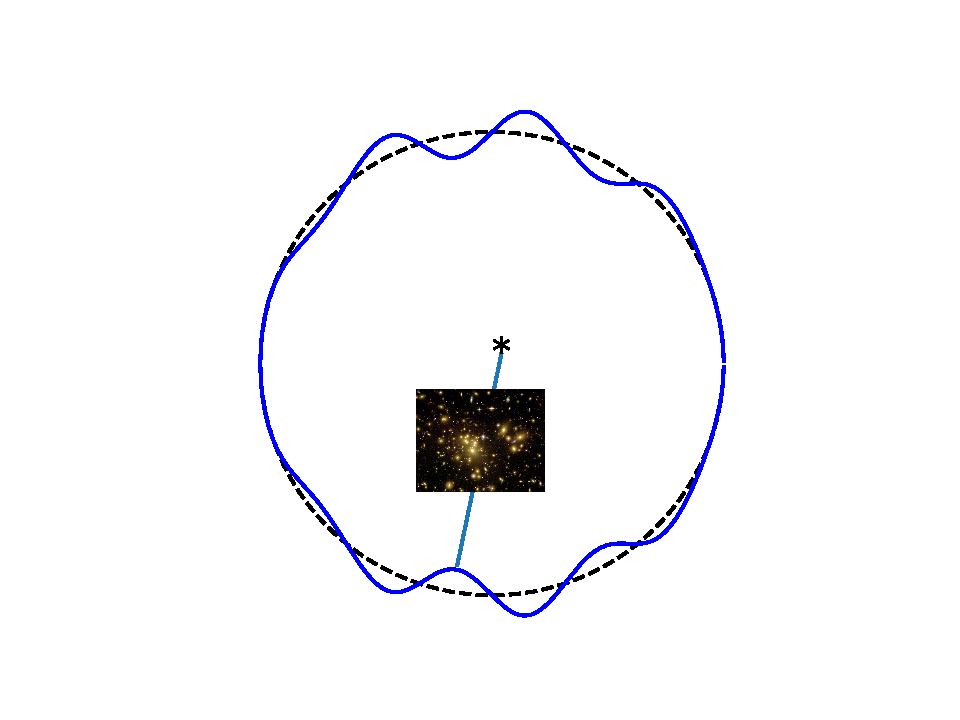
\includegraphics[width=0.4\textwidth]{td.pdf}
\caption{\footnotesize \label{fig:td}Schematic of the impact of time delays on the last scattering surface with us at the center. Dashed line denotes the assumed spherical last scattering surface, while blue solid curve denotes the more realistic corrugated surface due to time delays. Rays that pass through over-dense regions (as depicted in the figure) are slowed down; since all photons were released from the electrons at the same time, these ``slower'' photons travel shorter distances and therefore originated from closer distances than average..}
\end{wrapfigure}

Photons that comprise the CMB experience time delays or advances depending on the integrated potential through which they travel. Since photons do not decouple instantaneously from the electron-proton plasma, the surface of last scattering is often said to have a finite width; however, the directional-dependent change in the distance to last scattering is independent of its finite width and is a phenomenon different than the angular deflections that have been captured by recent experiments.

Although deflections and delays are two different phenomena, they share some similarities, especially in the case of the CMB. Both are determined by the integrated potential along the line of sight, although with slightly different kernels, as depicted in Figure~\rf{td}. It is clear that they will be highly correlated, so as a first approximation, we might view the maps of the lensing potential created for example in \citet{Aghanim:2018oex} as maps of distance to the last scattering surface. Another similarity, one that has not yet been exploited, is that the formalism first proposed in \citet{Hu:2001tn} can be applied to the delays as well, and this is what we will do in this paper. 